%%%%%%%%%%%%%%%%%%%%%%%%%%%%%%%%%%%%%%%%%%%%%%%%%%%%%%%%%%%
% --------------------------------------------------------
% Tau
% LaTeX Template
% Version 2.4.3 (01/09/2024)
%
% Author: 
% Guillermo Jimenez (memo.notess1@gmail.com)
% 
% License:
% Creative Commons CC BY 4.0
% --------------------------------------------------------
%%%%%%%%%%%%%%%%%%%%%%%%%%%%%%%%%%%%%%%%%%%%%%%%%%%%%%%%%%%

\documentclass[9pt,a4paper,twoside]{tau-class/tau}
\usepackage[english]{babel}

%----------------------------------------------------------
% TITLE
%----------------------------------------------------------

\journalname{Aprenentatge Computacional}
%% TODO: Optional, you can set a fancier title if you like
\title{Classificació de Supervivents del Titanic}

%----------------------------------------------------------
% AUTHORS, AFFILIATIONS AND PROFESSOR
%----------------------------------------------------------

%% TODO: Set your names here
\author[a,1]{Ricard Urpí Vilanova}
\author[b,2]{Ferran Villarta}
\author[c,3]{Natan Sisoev}

%----------------------------------------------------------

\affil[a]{1711326}
\affil[b]{1704051}
\affil[c]{1706198}

%----------------------------------------------------------
% FOOTER INFORMATION
%----------------------------------------------------------

\institution{Universitat Autònoma de Barcelona}
\footinfo{Pràctica Guiada}
\theday{\today}
\leadauthor{Group GPA-1} 		%% TODO: Set your group ID here
\course{Aprenentatge Computacional}

%----------------------------------------------------------
% ABSTRACT AND KEYWORDS
%----------------------------------------------------------

\begin{abstract}
Aquest treball presenta una anàlisi exhaustiva per a la classificació de supervivents del Titanic mitjançant tècniques d'aprenentatge automàtic. A partir d'un dataset amb informació sobre passatgers (classe, edat, sexe, tarifa, etc.), es realitza un preprocessament detallat que inclou imputació de valors perduts amb KNN, extracció de característiques com el deck de la cabina i títols dels noms, i normalització de dades. Es comparen 12 models diferents utilitzant Repeated Stratified K-Fold Cross Validation amb F1-score com a mètrica principal. El Gradient Boosting amb paràmetres optimitzats (learning rate 0.1, max depth 3, 201 estimators) obté els millors resultats amb un F1-score de 0.75 i AUC-ROC de 0.85, utilitzant només tres característiques: classe de passatger, tarifa i sexe. El model demostra un bon equilibri entre precisió i recall, amb capacitat de generalització adequada i sense sobreajust significatiu.
\end{abstract}

%----------------------------------------------------------

%% TODO: Set appropriate keywords for your report.
\keywords{Titanic, Aprenentatge automàtic, Gradient Boosting, Classificació, Cross Validation, F1-score, ROC-AUC}

%----------------------------------------------------------

\begin{document}
	%% Do NOT change any of this. Line numbers should be kept.
    \maketitle
    \thispagestyle{firststyle} \tauabstract
    \tableofcontents
    \linenumbers

%----------------------------------------------------------

\section{EDA (exploratory data analysis)}

Llegint i analitzant la base de dades vam veure que teniem les següents variables:

\begin{itemize}
    \item \textbf{PassengerId}: etiqueta, identifica a cada persona
    \item \textbf{Survived}: binària, 1 = sí, 0 = no
    \item \textbf{Pclass}: categòrica, 1 = primera, 2 = segona, 3 = tercera classe
    \item \textbf{Name}: etiqueta, nom de la persona (potser no únic)
    \item \textbf{Sex}: categòrica, female o male
    \item \textbf{Age}: numèrica, edat en anys
    \item \textbf{SibSp}: numèrica, nombre de germans o parelles en el Titanic
    \item \textbf{Parch}: numèrica, nombre de pares o fills en el Titanic
    \item \textbf{Ticket}: text, codi del tiquet
    \item \textbf{Fare}: numèrica, preu del tiquet
    \item \textbf{Cabin}: text, codi de la cabina
    \item \textbf{Embarked}: categòrica, port d'embarcació: C = Cherbourg, Q = Queenstown, S = Southampton
\end{itemize}

El target és l'atribut \textbf{Survived}, que pot prendre valors 0 o 1.

Ens faltaven dades, el port d'embarcació per a 2 persones, l'edat per a 177 i la cabina per a 687.

Analitzant les correlacions entre variables i la distribució de les dades no trobem grans inconvenients i ens cal acabar de seleccionar, normalitzar i processar les dades.

\begin{figure}[H]
    \centering
    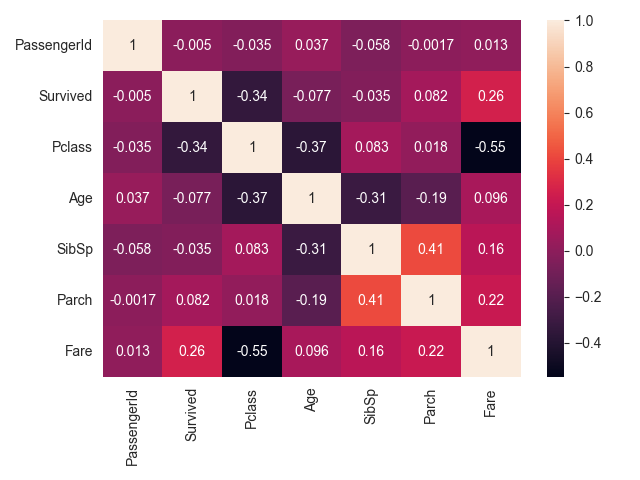
\includegraphics[width=0.4\textwidth]{figures/matriu_corr.png}
    \caption{Matriu de correlacions}
    \label{fig:exemple}
\end{figure}

\section{Preprocessing}

Per tractar les dades que ens falten hem començat per la cabina, considerem que és molt important per a la predicció, ho podem veure en la següent fotografia.

\begin{figure}[H]
    \centering
    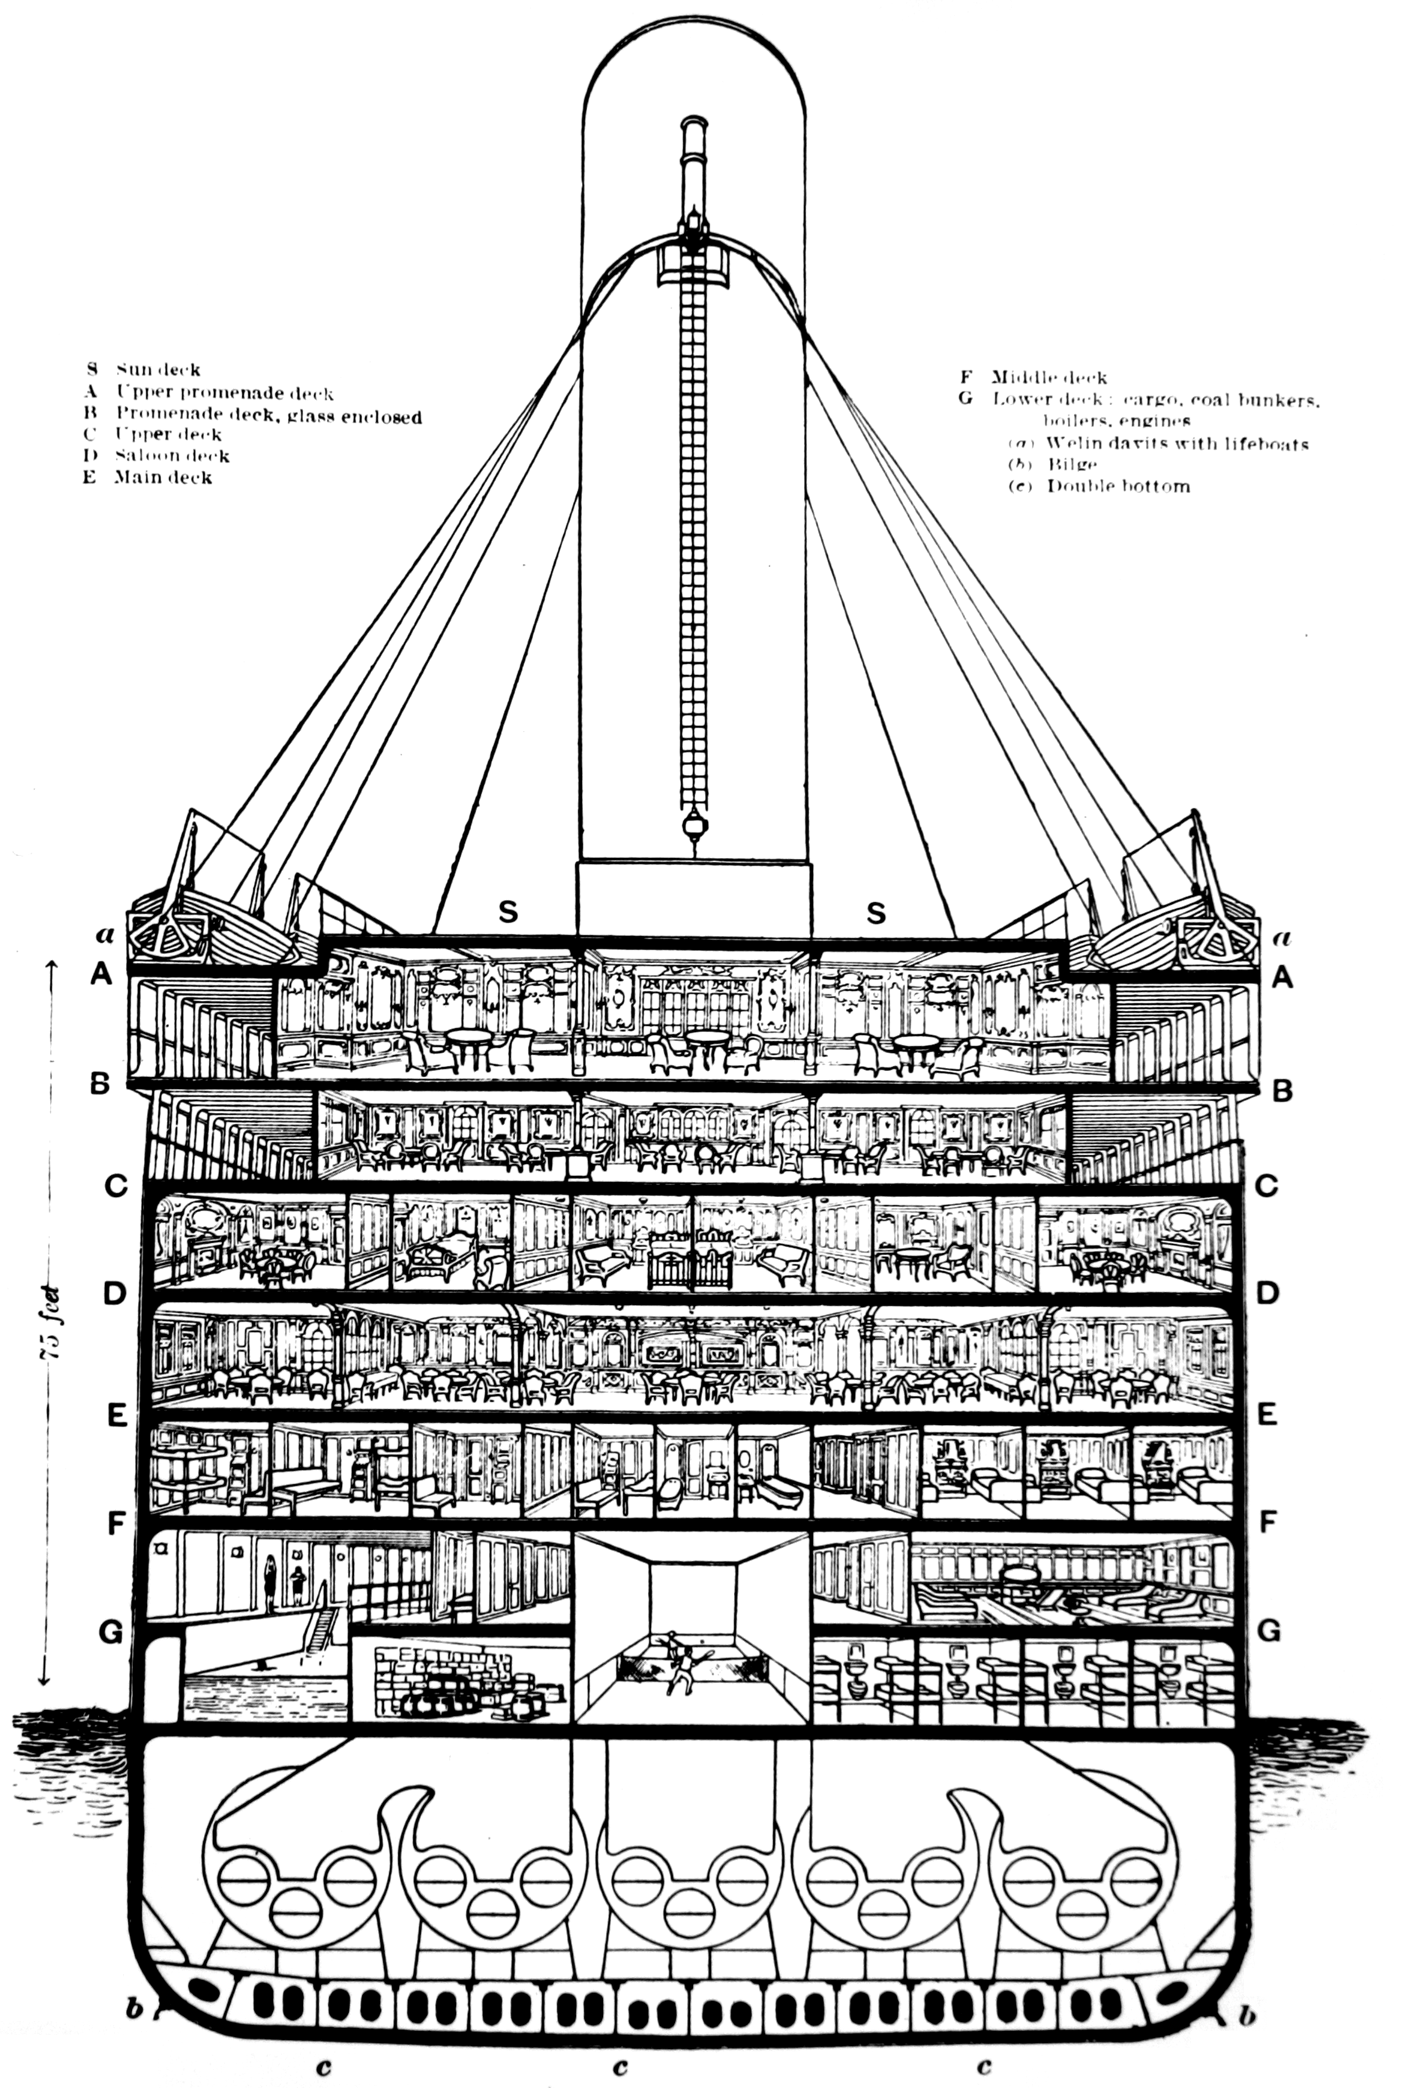
\includegraphics[width=0.2\textwidth]{figures/decks.png}
    \caption{Decks}
    \label{fig:exemple}
\end{figure}


Com ens falten moltes dades (aproximadament 80\% dels passatgers no tenen cabina) no té sentit assignar una cabina a cada passatger, hem creat una nova variable que conté la lletra del codi de la cabina i als passatgers que no en tenen els hem assignat una \textit{X}. Afegim una variable que indica si tenen cabina o no.
Als passatgers que no tenien port hem considerat que podíem mirar passatgers que tinguin preus de tiquets similars i assignar a aquests passatgers aquest port.
En el cas de l'edat hem decidit imputar les dades que ens falten (20\% aproximadament). La mitjana d'edat varia molt entre classes: les classes més pobres tenen una mitjana d'edat menor, així que hem creat una variable que ens indica el nombre de familiars (més familiars pot indicar una edat més baixa). A més, tots els noms tenen un títol i aquests corresponen majoritàriament a una certa franja d'edat, sexe...
Hem creat una variable amb el títol de cada persona. Aquest és un cas ideal per usar KNN i trobar passatgers similars per assignar una edat als que no tenen dades. Per això, considerem que les variables rellevants són \textbf{Fare}, \textbf{SibSp}, \textbf{Parch}, \textbf{FamilySize}, \textbf{Title}, \textbf{Cabin\_missing} i  \textbf{Pclass}.
Afegim variables binàries per indicar el deck (coberta que correspon a la lletra del codi del tiquet), el port d'embarcament i el sexe.
Finalment, tractem amb els \textit{outliers} i normalitzem les dades.
El nostre dataset ens queda amb les següents variables ja normalitzades: \textbf{Sex\_male}, \textbf{Embarked\_Q}, \textbf{Embarked\_S}, \textbf{Deck\_B}, \textbf{Deck\_C}, \textbf{Deck\_D},
\textbf{Deck\_E}, \textbf{Deck\_F}, \textbf{Deck\_G}, \textbf{Deck\_X}, \textbf{Title\_Military}, \textbf{Title\_Mr},
\textbf{Title\_Mrs}, \textbf{Title\_Ms}, \textbf{Title\_Nobility}, \textbf{Title\_Rev}, \textbf{Age}, \textbf{SibSp},
\textbf{Parch}, \textbf{Fare}, \textbf{FamilySize}, \textbf{Pclass}, \textbf{PassengerId}, \textbf{Survived} i
\textbf{Cabin\_missing}.

\section{Metric selection}

En aquest apartat hem seleccionat la mètrica que millor s'ajusta al nostre model.
\\\\
Després d'entrenar el model utilitzant regressió logística, obtenim les següents conclusions:

\begin{itemize}

\item \textbf{1. Accuracy}: Pot ser enganyosa en datasets desequilibrats.
   Encara que no és extremadament desequilibrat, hi ha més morts que supervivents.
   Així que un model que prediu gairebé sempre "mor" tindria bona accuracy, però no seria bo per detectar supervivents.

\item \textbf{2. Precision i Recall}: Precision mira quants  supervivents predits realment sobreviuen (minimitza falsos positius).
\\ Recall mira quants  supervivents reals hem detectat (minimitza falsos negatius).
\\Per comparar models cal un equilibri entre ambdues.

\item \textbf{3. Average Precision Score}: Resumeix tota la Precision-Recall curve.
   És útil quan el model retorna probabilitats i hi ha molts casos positius escassos.
   En aquest cas les classes no són extremadament desequilibrades.

\item \textbf{4. ROC-AUC}: També resumeix la capacitat del model per separar classes.
   Però dona menys informació en casos desequilibrats, pot donar una falsa sensació de bon rendiment quan hi ha molts negatius.

\item \textbf{5. F1-score}: Combina Precision i Recall en una mitjana, equilibrant la capacitat de detectar supervivents (recall) i no predir falsament supervivents (precision).

\end{itemize}

Per aquests motius, hem triat l'F1-score com a mètrica principal per avaluar els models.

\begin{figure}[H]
    \centering
    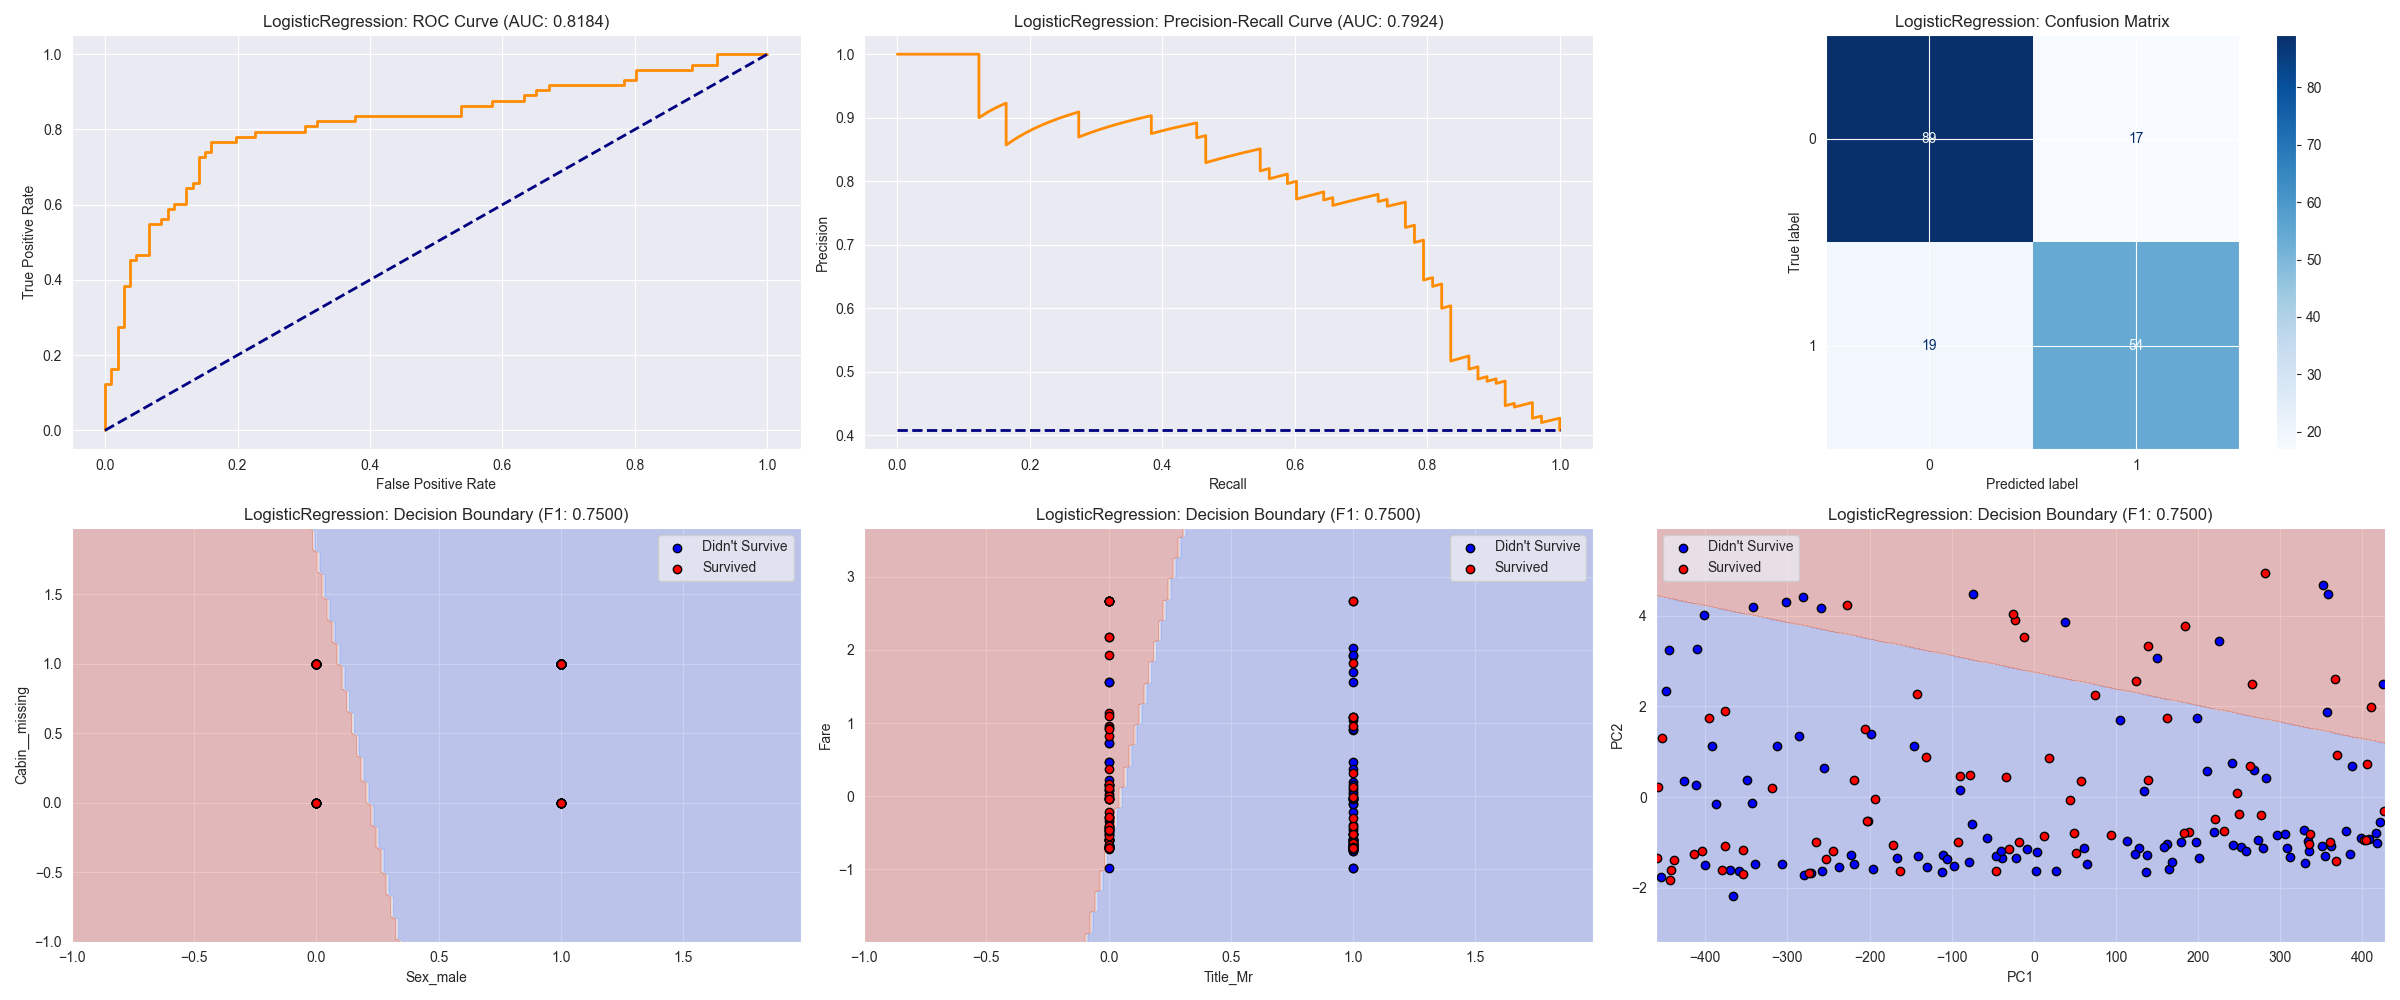
\includegraphics[width=0.4\textwidth]{figures/punt3.png}
    \caption{Gràfics}
    \label{fig:exemple}
\end{figure}

Podem observar com hem generat diferents gràfics representant les dues corbes, la matriu de confusió, les fronteres per dues parelles de features i PCA.

\section{Model Selection amb Crossvalidation}

Els mètodes que hem provat per fer validació creuada han estat: K-Fold, Stratified K-Fold, Repeated Stratified K-Fold i Shuffle \& Split. Els hem provat tots amb cadascun dels mètodes que presentarem a continuació. Com és un dataset petit, hem decidit escollir el més robust tot i tardar una mica més: Repeated Stratified K-Fold. L'implementem directament en la nostra classe \texttt{Metrics}, de manera que qualsevol testeig que fem serà fent servir aquest tipus de validació creuada.

Seleccionem els següents models:
\begin{itemize}
    \item \textbf{Logistic Regression}
    \item \textbf{KNN}
    \item \textbf{Gradient Descent}
    \item \textbf{Random Forest}
    \item \textbf{Extra Trees}
    \item \textbf{Support Vector Machine}
    \item \textbf{LinearSVC}
    \item \textbf{Gradient Boosting}
    \item \textbf{Naive Bayes}
    \item \textbf{Perceptron}
    \item \textbf{Passive Agressive}
    \item \textbf{Neural Network}
\end{itemize}

Els més adequats són Random Forest, Extra Trees i Gradient Boosting, que gestionen bé petites mostres i desequilibris. Models lineals com Logistic Regression i SVC poden funcionar si les dades estan normalitzades, mentre que Perceptron i Passive Aggressive són menys útils. Altres com KNN, Naive Bayes o MLPClassifier poden donar resultats raonables però requereixen cura amb els hiperparàmetres o tenen risc d’\textit{overfit}.



\begin{figure}[H]
    \centering
    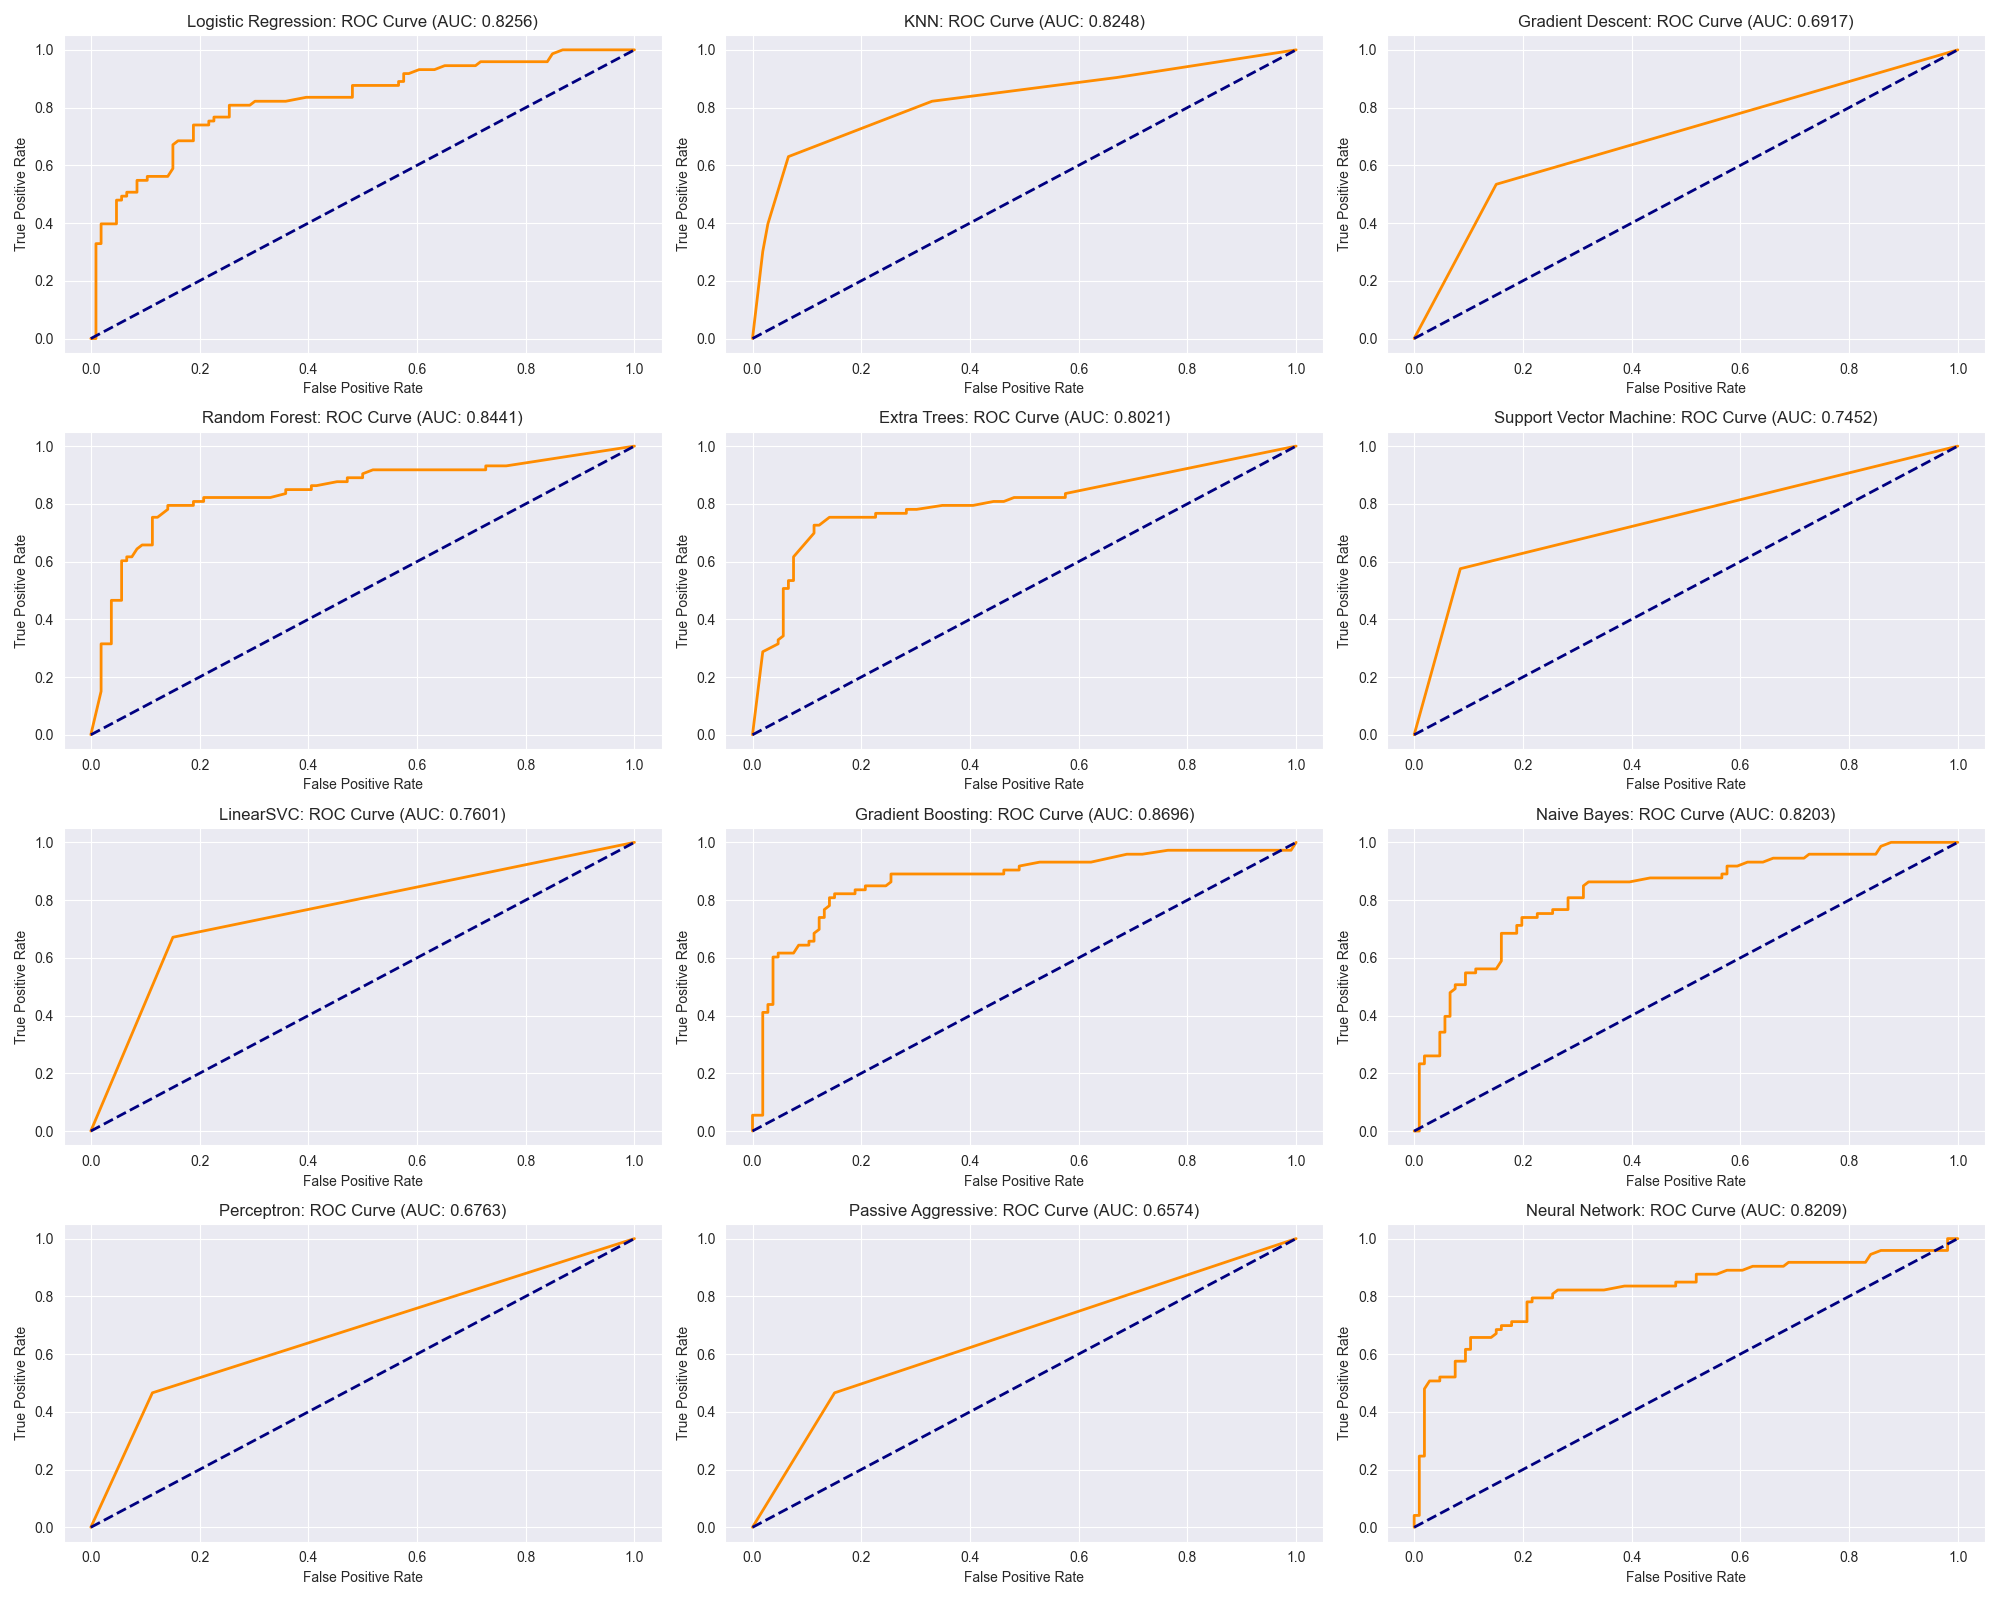
\includegraphics[width=0.4\textwidth]{figures/red_dims.png}
    \caption{Corbes amb el dataset reduït}
    \label{fig:exemple}
\end{figure}

Hem provat a reduir la dimensionalitat del model per veure si obteníem bons resultats en dimensions menors que poguéssim visualitzar. Aquests és un dels molts resultats visuals que hem obtingut:

\begin{table}[ht]
\centering
\tiny % mida de lletra mínima
\setlength{\tabcolsep}{2pt} % redueix espai entre columnes
\resizebox{0.48\textwidth}{!}{% lleugerament menys que la meitat
\begin{tabular}{l c p{3.6cm}} % tercera columna amb ample fix
\hline
\textbf{Model} & \textbf{Mean} & \textbf{Best Params} \\
\hline
Logistic Reg. & 0.7106 & C=1, max\_iter=1000, penalty=l2 \\
KNN & 0.7098 & metric=euclidean, n\_neighbors=9 \\
Grad. Descent & 0.7109 & alpha=0.001, eta0=0.01, lr=optimal \\
Random Forest & 0.7042 & max\_depth=5, n\_estimators=101 \\
Extra Trees & 0.7101 & max\_depth=2, n\_estimators=51 \\
SVM & 0.7101 & C=0.1, gamma=scale, kernel=linear \\
LinearSVC & 0.7101 & C=0.1, loss=hinge \\
\textbf{Grad. Boost.} & \textbf{0.7265} & lr=0.1, max\_depth=3, n\_estimators=201 \\
Naive Bayes & 0.7164 & var\_smoothing=1e-12 \\
Perceptron & 0.6108 & alpha=1e-05, eta0=0.1 \\
Passive Agg. & 0.7101 & C=0.001, max\_iter=1000 \\
Neural Net & 0.7093 & act=tanh, alpha=1e-05, lr=const. \\
\hline
\end{tabular}
}
\caption{Comparació de models i paràmetres òptims.}
\label{tab:model_params_small}
\end{table}

\begin{figure}[H]
    \centering
    \includegraphics[width=0.4\textwidth]{figures/RF_Fare_Sex_male.png}
    \caption{Random Forest amb variables Fare i Sex\_male}
    \label{fig:exemple}
\end{figure}

Per trobar els millors hiperparàmetres hem fet una cerca provant-ne diferents combinacions, ja que el dataset és relativament petit. Hem pogut obtenir la següent taula:

\begin{table}[ht]
\centering
\tiny % mida de lletra mínima
\setlength{\tabcolsep}{1.5pt} % redueix espai entre columnes
\resizebox{0.48\textwidth}{!}{% adapta a mitja pàgina
\begin{tabular}{l c p{3.4cm}} % tercera columna amb ample fix
\hline
\textbf{Model} & \textbf{Mean Test Score} & \textbf{Best Parameters} \\
\hline
Logistic Reg. & 0.7106 & C=1, max\_iter=1000, penalty=l2 \\
KNN & 0.7098 & metric=euclidean, n\_neighbors=9, weights=uniform \\
Grad. Descent & 0.7109 & alpha=0.001, eta0=0.01, lr=optimal \\
Random Forest & 0.7042 & max\_depth=5, n\_estimators=101 \\
Extra Trees & 0.7101 & max\_depth=2, n\_estimators=51 \\
SVM & 0.7101 & C=0.1, gamma=scale, kernel=linear \\
LinearSVC & 0.7101 & C=0.1, loss=hinge, max\_iter=1000 \\
\textbf{Grad. Boost.} & \textbf{0.7265} & lr=0.1, max\_depth=3, n\_estimators=201 \\
Naive Bayes & 0.7164 & var\_smoothing=1e-12 \\
Perceptron & 0.6108 & alpha=1e-05, eta0=0.1, max\_iter=1000 \\
Passive Agg. & 0.7101 & C=0.001, max\_iter=1000 \\
Neural Net & 0.7093 & act=tanh, alpha=1e-05, lr=adaptive, max\_iter=1000 \\
\hline
\end{tabular}
}
\caption{Comparació de models amb els millors hiperparàmetres i el seu \textit{mean test score}.}
\label{tab:model_params_small}
\end{table}

\section{Anàlisi Final}

\textbf{Resultats finals del model:}
S'han explorat totes les combinacions possibles de \textit{features} per determinar si era possible millorar el rendiment eliminant informació redundant. Els resultats indiquen que l'\textit{score} augmenta de \textbf{0.726538} a \textbf{0.749594} quan s'utilitzen només les variables \textit{[Pclass, Fare, Sex\_male]}. Aquest conjunt de tres característiques proporciona la informació més rellevant per al model, reduint-ne la complexitat i millorant la capacitat de generalització. Per aquest motiu, hem decidit conservar només aquestes columnes, i els gràfics i comentaris finals que segueixen es basen en aquesta versió definitiva del model.

\begin{figure}[H]
    \centering
    \includegraphics[width=0.4\textwidth]{figures/Captura de pantalla 2025-10-27 234726.png}
    \caption{Corba AUC-ROC del Gradient Boosting}
    \label{fig:roc_gb}
\end{figure}

\begin{figure}[H]
    \centering
    \includegraphics[width=0.4\textwidth]{figures/Captura de pantalla 2025-10-27 234751.png}
    \caption{Corba Precision-Recall del Gradient Boosting}
    \label{fig:pr_gb}
\end{figure}

\begin{table}[H]
\centering
\scriptsize
\begin{tabular}{|l|l|l|l|l|l|}
\hline
\textbf{Accuracy} & \textbf{Precision} & \textbf{Recall} & \textbf{F1-score} & \textbf{AUC-ROC} & \textbf{AUC-PR} \\
\hline
0.8044 & 0.8392 & 0.6438 & 0.7496 & 0.8535 & 0.8299 \\
\hline
\end{tabular}
\caption{Mètriques finals del model Gradient Boosting.}
\label{tab:metrics_gb}
\end{table}

\textbf{1. Avaluació de mètriques:}
La mètrica que menys ens agrada és el \textbf{recall}, ja que és força baixa (0.64) en comparació amb la \textbf{precision} (0.84). Això indica que el model tendeix a identificar bé els supervivents que prediu, però en deixa escapar alguns (falsos negatius). És a dir, és més “conservador” a l’hora de predir supervivència.
Això pot ser conseqüència d’un desequilibri lleu entre classes i del fet que treballem amb poques mostres. Recordem que les mètriques s’han obtingut mitjançant \textit{validació creuada}, i el conjunt de dades limitat incrementa la variabilitat dels resultats.

\textbf{2. Interpretació global del rendiment:}
El \textbf{F1-score de 0.75} reflecteix un bon equilibri entre \textit{precision} i \textit{recall}, però no és un resultat excepcional. Esperàvem un valor una mica superior, però tenint en compte que el model està ben regularitzat i que s’ha evitat l’\textit{overfitting}, considerem que el rendiment és satisfactori dins de les limitacions del dataset.
El \textbf{ROC-AUC de 0.85} i el \textbf{PR-AUC de 0.83} mostren una bona capacitat de discriminació entre classes, amb corbes suaus i coherents (Figures \ref{fig:roc_gb} i \ref{fig:pr_gb}).

\textbf{3. Conclusions sobre el model:}
El \textbf{Gradient Boosting} s’ha mostrat com el model més robust i estable, amb una bona gestió del \textit{bias-variance tradeoff}. Els hiperparàmetres triats (\texttt{learning\_rate = 0.1}, \texttt{max\_depth = 3}, \texttt{n\_estimators = 201}) proporcionen un bon equilibri entre rendiment i generalització, evitant sobreajustar-se a les dades d’entrenament.

\textbf{4. Marge de millora:}
Encara que el model és sòlid, hi ha espai per optimitzar-lo:

\begin{itemize}
    \item \textbf{Feature engineering:} Analitzar i ajustar les variables d’entrada segons el model, com combinacions d’edat, títol i classe.
    \item \textbf{Hiperparàmetres:} Explorar altres paràmetres com \texttt{min\_samples\_leaf}, \texttt{subsample} o \texttt{max\_features} per millorar generalització i \textit{recall}.
    \item \textbf{Més dades o augment:} Ampliar el dataset o aplicar tècniques com \textit{SMOTE} per equilibrar les classes i millorar el \textit{recall}.
    \item \textbf{Models avançats:} Provar alternatives com \textbf{XGBoost} o \textbf{LightGBM} per possible millora de rendiment.
\end{itemize}

\textbf{5. Conclusió final:}
Tot i les seves limitacions, el nostre model de \textbf{Gradient Boosting} aconsegueix un rendiment sòlid i estable, amb un bon balanç entre \textit{precision} i \textit{recall}. Les mètriques obtingudes mostren que el model generalitza correctament i no pateix sobreajustament greu, convertint-lo en una opció adequada per a problemes de classificació binària amb dades reduïdes, com el del Titanic.



\end{document}